% Provenance (never printed): see sources/outline_sources.md (Year 2: taphonomy; index fossils;
% facies and fossils as environment markers; reconstructing a palaeoenvironment from a map and a
% section). Taphonomy after Loron (2024); live, dead and fossil assemblages after Tyler and
% Kowalewski (2025); Lagerstaetten after Gaines and others (2024), Mussini and Butterfield
% (2025), Vannier and others (2018), Gerschermann and others (2021) and Rauhut and others
% (2018); zone durations after Al-Suwaidi and others (2022); ichnofacies after Buatois and others
% (2020) and Paz and others (2023); stenohaline groups after McGairy and others (2021) and Saleh
% and others (2022). The Varden column from figdata/shared/region.py; porosities and rates from
% figdata/bachelor-2/palaeoenv.py; exercise and problem values in the Book 4 scratch calculator
% calc/ch20.py. The fossil content given to the Varden units is invented, like the region.
\chapter{जीवाश्म और पुरापर्यावरण}\label{ch:b2:palaeoenvironments}

धूसर बलुआ पत्थर की एक पटिया पर तीन सुराग पड़े हैं: वह लकीर जो किसी ट्राइलोबाइट ने कीचड़ में जोतते हुए बनाई,
वे लहरिकाएँ जो कोई धारा पीछे छोड़ गई, और एक बिल जिसे किसी कृमि ने खोदा और छोड़ दिया। इनमें से कोई भी
पूरा जानवर नहीं है, फिर भी मिलकर वे बताते हैं कि यह पहाड़ी ढलान कभी एक समुद्र का तल थी, इतना उथला
कि लहरें उसे हिला सकें, इतना खारा कि ट्राइलोबाइट उसमें रह सकें। जीवाश्म बीते जीवन के
अवशेष और चिह्न हैं, और भूविज्ञानी उन्हें दो बार पढ़ते हैं: घड़ियों की तरह जो चट्टान की आयु बताती हैं,
और उस स्थान के साक्षियों की तरह जहाँ वह बनी। यह अध्याय एक जीवित वस्तु का उसकी मृत्यु से
संग्रहकर्ता की दराज़ तक अनुसरण करता है, उन दुर्लभ निक्षेपों को खोलता है जहाँ कोमल शरीर तक बचे रहते हैं, और फिर
वार्डन पहाड़ियों के आवरण में एक लुप्त समुद्र के पर्यावरण को, संख्याओं के साथ, पढ़ता है।
% ledger: usgs:fossil-record-bulk, loron24:taphonomy

\begin{recall}
\textbf{स्कूल की पुस्तकों से}: जीवाश्म, साँचा, ढलाई और \omterm{def:b2:palaeoenvironments:fossil-kinds}{चिह्न जीवाश्म}; दफ़न और खनिज किसी सीपी को
पत्थर में कैसे बदलते हैं; समय के साथ जीवाश्मों का अनुक्रम। \textbf{पुस्तक 3 (स्नातक वर्ष 1) से}:
अवसादी फ़ेसीज़ और निक्षेपण-परिवेश, गंदलाव-निक्षेप, भित्तियाँ और ऊइड; जैव-क्षेत्र, सूचक
जीवाश्म और पहली उपस्थिति के आँकड़े; संपीड़न, डिकंपैक्शन, एथी का नियम और किसी परत की ठोस
मोटाई; सीमेंट; आवास-स्थान। \textbf{पिछले अध्यायों से}: ट्रांसग्रेशन और रिग्रेशन,
दीर्घकालिक समुद्र-स्तर और महासागरीय अनॉक्सी घटनाएँ (\cref{ch:b2:phanerozoic-earth})। प्रजातियाँ
कैसे विकसित होती हैं, और जंतुओं तथा पादपों का वर्गीकरण कैसे होता है, ये जीवविज्ञान की पुस्तकों के विषय हैं।
\end{recall}

\section{मृत्यु से जीवाश्म तक}\label{sec:b2:palaeoenvironments:taphonomy}

अधिकांश जीवित वस्तुएँ पीछे कुछ नहीं छोड़तीं। जीवाणु और मृतभक्षी कोमल भागों को दिनों या वर्षों में
खा जाते हैं, धाराएँ कठोर भागों को तोड़ती और बिखेरती हैं, और मृदाओं तथा छिद्र-जल के अम्ल
जो बचा है उसे घोल देते हैं। जीवाश्म वह है जो इन सबसे बच निकलता है, और फिर उसे धारण करने वाली चट्टान के
दफ़न, तापन और उत्थान से भी बचता है।

\begin{definition}[टैफ़ोनॉमी; परिरक्षण-संभाविता]\label{def:b2:palaeoenvironments:taphonomy}
\emph{टैफ़ोनॉमी}\index{टैफ़ोनॉमी} इस बात का अध्ययन है कि किसी जीव के अवशेषों के साथ
उसकी मृत्यु से जीवाश्म के रूप में उसकी खोज तक क्या होता है: अपघटन, मृतभक्षण, परिवहन, दफ़न, और
डायाजेनेसिस के रासायनिक परिवर्तन। किसी जीव की, या उसके किसी भाग की, \emph{परिरक्षण-संभाविता}\index{परिरक्षण-संभाविता}
वह प्रायिकता है कि वह इन चरणों से गुज़रे
और चट्टान में बचा रहे।
\end{definition}
% ledger: loron24:taphonomy

हर चरण कुछ हटाता है, कुछ जोड़ता है, या कुछ बदलता है। अपघटन और मृतभक्षण कोमल
ऊतकों को हटाते हैं; छिद्र-जल के खनिज किसी हड्डी के छिद्रों को भरते हैं या किसी
सीपी के ऐरागोनाइट को प्रतिस्थापित करते हैं, ऐसा पदार्थ जोड़ते हुए जो जानवर के पास कभी नहीं था; तापन बचे हुए कार्बनिक अणुओं को बदल देता है।
लोरॉन इन सभी मरणोपरांत परिवर्तनों को तीन प्रकारों में बाँटते हैं, लाभ, हानि और परिवर्तन, और
उन्हें किसी जीव और उसके जीवाश्म के बीच किसी भी मापने योग्य लक्षण के परिवर्तन के लिए एक समीकरण के रूप में
लिखते हैं। नीचे का चित्र चरणों का अनुसरण करता है और दिखाता है कि हर एक क्या छीन लेता है।
% ledger: loron24:taphonomy

\begin{omfigure}
\centering
\begin{tikzpicture}[font=\scriptsize, x=1cm, y=1cm,
  stage/.style={draw=black!60, fill=omSea!12, rounded corners=2pt, align=center,
    text width=2.05cm, minimum height=1.25cm, inner sep=2pt},
  loss/.style={align=center, text width=2.05cm, text=omThm!80!black}]
\node[stage] (a) at (0,0) {\textbf{मृत्यु}\\एक जीवित\\समुदाय};
\node[stage] (b) at (2.75,0) {\textbf{अपघटन और}\\\textbf{मृतभक्षण}\\तल पर};
\node[stage] (c) at (5.5,0) {\textbf{परिवहन}\\धाराएँ छाँटती\\और तोड़ती हैं};
\node[stage] (d) at (8.25,0) {\textbf{दफ़न}\\सक्रिय परत\\के नीचे};
\node[stage] (e) at (11,0) {\textbf{डायाजेनेसिस}\\संपीड़न,\\प्रतिस्थापन};
\node[stage] (f) at (13.75,0) {\textbf{अनावरण}\\और\\संग्रह};
\foreach \u/\v in {a/b, b/c, c/d, d/e, e/f} {\draw[-{Stealth[length=2mm]}, black!70] (\u) -- (\v);}
\node[loss, anchor=north] at (2.75,-0.8) {कोमल ऊतक नष्ट;\\कंकाल बिखर जाते हैं};
\node[loss, anchor=north] at (5.5,-0.8) {हल्के भाग बह जाते हैं,\\सीपियाँ टूटती हैं};
\node[loss, anchor=north] at (8.25,-0.8) {धीमा दफ़न: हानियों\\के लिए अधिक समय};
\node[loss, anchor=north] at (11,-0.8) {ऐरागोनाइट घुला,\\खनिज जुड़े};
\node[loss, anchor=north] at (13.75,-0.8) {अपरदित हो गए,\\या कभी मिले नहीं};
\end{tikzpicture}
\par\smallskip{\small एक जीवित समुदाय से एक संग्रह तक का टैफ़ोनॉमिक मार्ग, और हर चरण
क्या हटाता या बदलता है। दफ़न निर्णायक मोड़ है: उससे पहले अवशेष हर हानि के सामने
खुले रहते हैं; उसके बाद केवल डायाजेनेसिस और अपरदन उन पर कार्य करते हैं।}
\end{omfigure}
% ledger: loron24:taphonomy

स्कूल की पुस्तकों ने चट्टान में सुरक्षित बीते जीवन के किसी भी अवशेष या चिह्न को जीवाश्म कहा। ये दो प्रकार
चट्टान में इतना भिन्न व्यवहार करते हैं कि वे अपने-अपने नामों के पात्र हैं।

\begin{definition}[काय जीवाश्म; चिह्न जीवाश्म]\label{def:b2:palaeoenvironments:fossil-kinds}
एक \emph{काय जीवाश्म}\index{काय जीवाश्म} किसी जीव के शरीर का भाग है, या उस भाग का साँचा या ढलाई:
सीपी, हड्डी, दाँत, पत्ती, और दुर्लभ निक्षेपों में कोई कोमल ऊतक। एक
\emph{चिह्न जीवाश्म}\index{चिह्न जीवाश्म} वह संरचना है जिसे किसी जीव ने किसी अवसाद या चट्टान के भीतर या
उस पर अपनी गतिविधि से बनाया: पदचिह्न, घिसटने की लकीर, बिल, छेद, भोजन का कोई प्रतिरूप।
\end{definition}

\omterm{def:b2:palaeoenvironments:fossil-kinds}{चिह्न जीवाश्म} उसी अवसाद का भाग है जिसमें वह खोदा गया: उसे खिसकाने वाली धारा उसे नष्ट कर देती।
इसलिए वह ठीक उसी स्थान की परिस्थितियाँ दर्ज करता है जहाँ उसका निर्माता रहता था, जो एक सीपी,
जो तल पर आसानी से लुढ़क जाती है, सदा नहीं करती। \omterm{def:b2:palaeoenvironments:fossil-kinds}{चिह्न जीवाश्मों} के नाम जीवों की तरह रखे जाते हैं, एक
वंश और एक प्रजाति के साथ, पर नाम संरचना का वर्णन करता है, जानवर का नहीं: वही बिल
कई प्रकार के जानवर खोद सकते हैं, और एक जानवर कई प्रकार के चिह्न छोड़ सकता है।

\subsection*{दफ़न बनाम विनाश}

दफ़न और विनाश की दौड़ को एक सरल मॉडल में रखा जा सकता है। तल पर पड़े अवशेष
एक स्थिर दर $k$ से नष्ट होते हैं, यानी प्रति इकाई समय वह प्रायिकता कि वे खा लिए जाएँ,
टूट जाएँ या घुल जाएँ; अवसाद की मोटाई $h$ से ढकते ही वे सुरक्षित हैं; और
अवसाद दर $s$ से जमा होता है।

\begin{proposition}[विनाश से पहले दफ़न]\label{prop:b2:palaeoenvironments:burial}
इन मान्यताओं के अंतर्गत, किसी अवशेष के सुरक्षा तक पहुँचने की प्रायिकता है
\[
  P = e^{-kh/s}.
\]
यह तीनों राशियों पर केवल दफ़न तक के समय, $h/s$, और
तल पर माध्य उत्तरजीविता-काल, $1/k$, के अनुपात के माध्यम से निर्भर करती है।
\end{proposition}

\begin{proof}
अवशेष को समय $T = h/s$ चाहिए, मोटाई $h$ से ढकने के लिए। विनाश की स्थिर दर
$k$ के साथ, बचे रहने की प्रायिकता $p(t)$, समय $t$ तक, समीकरण $p' = -kp$, $p(0) =
1$ का पालन करती है, जिससे $p(t) = e^{-kt}$; $t = T$ पर यह $e^{-kh/s}$ है।
\end{proof}

\begin{example}[एक शांत तल पर एक सीपी]\label{ex:b2:palaeoenvironments:shell}
मान लीजिए एक सीपी तल पर औसतन 20 वर्ष बची रहती है, $k = \qty{0.05}{yr^{-1}}$, और
$h = \qty{0.1}{m}$ कीचड़ के नीचे सुरक्षित है। $s = \qty{1}{mm.yr^{-1}}$ पर दफ़न तक का समय 100
वर्ष है और $P = e^{-5} = 0.0067$: सौ में एक से भी कम सीपी बचती है।
\qty{1}{cm.yr^{-1}} पर, $P = e^{-0.5} = 0.61$। एक दिन में \qty{0.3}{m} रेत डाल देने वाला तूफ़ान
सब कुछ एक साथ दबा देता है, और तब $P$ एक के निकट होता है। संख्याएँ मान ली गई हैं, पर सीख
नहीं: जीवाश्म वहाँ एकत्र होते हैं जहाँ अवसाद तेज़ी से या अचानक परतों में आता है।
\end{example}

मॉडल यह भी दिखाता है कि अभिलेख पक्षपाती क्यों है। एक कोमल-शरीर कृमि, जिसका तल पर माध्य उत्तरजीविता-काल
दशकों के बजाय दिनों का है, उसका $k$ किसी मोटी सीपी से सैकड़ों गुना बड़ा होता है,
और इसलिए उसकी संभावना चरघातांकी रूप से छोटी। जीवाश्म अभिलेख का अधिकांश भाग कवचधारी जंतुओं
और सूक्ष्म अवशेषों से बना है। टायलर और कोवालेव्स्की ने जाँचा कि एक समुदाय चट्टान तक
पहुँचते-पहुँचते कितना खोता है। एक तटीय समुद्र-तल के 51 स्थलों पर उन्होंने अकशेरुकियों की 135 जीवित प्रजातियाँ
गिनीं, तल पर मृत पड़ी सीपियों और कंकालों में 150 प्रजातियाँ, और 112 ऐसी जिनका
जीवाश्म अभिलेख भी है। मृत जीवितों से अधिक हैं क्योंकि तल पर सीपियाँ
अनेक वर्षों में एकत्र हुईं, उन जंतुओं से जो अब वहाँ नहीं रहते। अपरदभक्षी और मांसाहारी, अधिकतर
कोमल-शरीर, सबसे कम परिरक्षित होते हैं; फिर भी जीवित समुदाय के मुख्य पारिस्थितिक समूह
सभी मृतों में फिर से मिले।
% ledger: usgs:fossil-record-bulk, tyler25:live-dead, tyler25:soft-bodied

\section{असाधारण परिरक्षण की खिड़कियाँ}\label{sec:b2:palaeoenvironments:lagerstatten}

\begin{definition}[लागरश्टेटे]\label{def:b2:palaeoenvironments:lagerstatte}
एक \emph{लागरश्टेटे}\index{लागरश्टेटे} (बहुवचन लागरश्टेटेन) वह अवसादी निक्षेप है जो
असाधारण गुणवत्ता के जीवाश्म परिरक्षित करता है, विशेषकर वे कोमल, अजैवखनिजित ऊतक जिन्हें
अपघटन लगभग हर अन्य स्थान पर नष्ट कर देता है; ऐसे निक्षेप को कॉन्सर्वाट-लागरश्टेटे भी कहते हैं।
\end{definition}
% ledger: gaines24:konservat

लागरश्टेटेन दुर्लभ हैं, पर कोमल-शरीर जंतुओं के बारे में जो ज्ञात है उसका बड़ा भाग उन्हीं से आता है, और
जंतुओं का पहला महान विकिरण, कैम्ब्रियन में, उन्हीं से सबसे अच्छी तरह समझा जाता है।
% ledger: gaines24:konservat

\subsection*{बर्जेस शेल}

1909 में चार्ल्स वॉलकॉट ने अपनी क्षेत्र-पुस्तिका में एक छोटे संधिपाद का रेखाचित्र बनाया जो उन्हें ब्रिटिश कोलंबिया के
बर्जेस शेल में मिला था। बाद में उन्होंने उसके सैकड़ों
नमूने, \emph{वैप्टिया}, लगभग \qty{2}{m} मोटे एक ही अंतराल से एकत्र किए, फ़िलोपॉड
संस्तर से; उसका आधुनिक वर्णन दो संग्रहालयों में रखे 1800 से अधिक नमूनों पर टिका है। बर्जेस
शेल, लगभग 508 मिलियन वर्ष पुराना, गहरे जल में, एक खड़े जलमग्न
कगार के सामने जमा हुआ था। उसके जीवाश्मों में कवचहीन जंतु हैं, जो कार्बन की चपटी परतों के रूप में परिरक्षित हैं,
प्रायः पूरे शरीर। ऐसा परिरक्षण ऑक्सीजन-विहीन कीचड़ में दफ़न से जुड़ा है जिसमें जंतुओं ने
बिल नहीं खोदे और धाराओं ने जिसे फिर नहीं उलटा-पलटा: ऊपर के चित्र की हानियाँ तुरंत रुक गईं।
% ledger: vannier18:waptia, mussini25:burgess

\begin{omfigure}
\centering
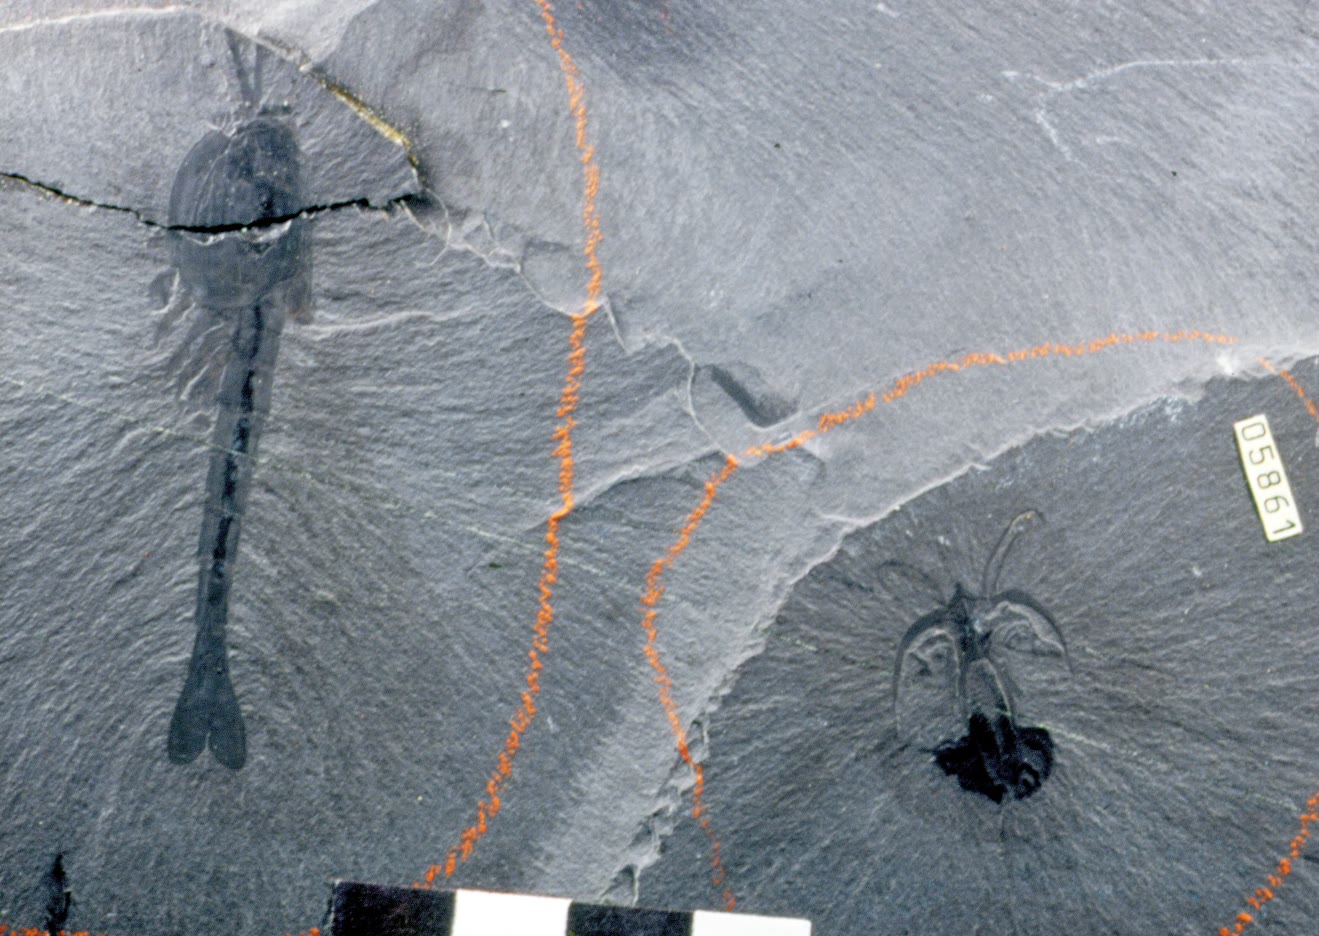
\includegraphics[width=0.72\linewidth]{images/book4/b2-20-burgess-waptia-marrella.jpg}
\par\smallskip{\small बर्जेस शेल के दो संधिपाद, कार्बन की गहरी परतों के रूप में परिरक्षित:
\emph{वैप्टिया} (बाएँ) और \emph{मरेला} (दाएँ)। (James
St.~John, CC~BY~2.0, विकिमीडिया कॉमन्स के माध्यम से।)}
\end{omfigure}
% ledger: mussini25:burgess

\subsection*{सोल्नहोफ़ेन}

बवेरिया में सोल्नहोफ़ेन और आइख़श्टेट के महीन कणों वाले चूना-पत्थर लैगूनों में जमा हुए,
टिथोनियन के आरंभ में, जो जुरैसिक का अंतिम युग है और \qty{149.2}{Ma} पहले आरंभ हुआ। वे
\emph{आर्कियोप्टेरिक्स} के बारह नमूनों, अनेक टेरोसॉरों और उन मछलियों के प्रारूप-स्थल हैं
जिनके कोमल ऊतक और रंग-प्रतिरूप तक बचे हैं। वहाँ जीवाश्म दुर्लभ हैं, पर उनका
परिरक्षण उत्कृष्ट है। कई परिस्थितियाँ प्रस्तावित की गई हैं, जो शायद साथ-साथ कार्य करती थीं:
तल का जल समुद्री जल से लगभग तीन गुना खारा या अत्यधिक क्षारीय, जो जीवाणु-अपघटन को
धीमा करता है; जीवाणुओं की चटाइयाँ जिन्होंने शवों को बंद कर दिया; ऑक्सीजन-रहित तल-जल, जिसने
मृतभक्षियों को दूर रखा; और तूफ़ान जिन्होंने चूने की कीचड़ को हिलाया और शवों को शीघ्र दबा दिया। इनमें से
हर एक उत्तरजीविता-काल $1/k$ को बढ़ाती है या दफ़न तक के समय $h/s$ को घटाती है।
% ledger: gerschermann21:solnhofen, rauhut18:archaeopteryx, ics4:jurassic-stages

\begin{omfigure}
\centering
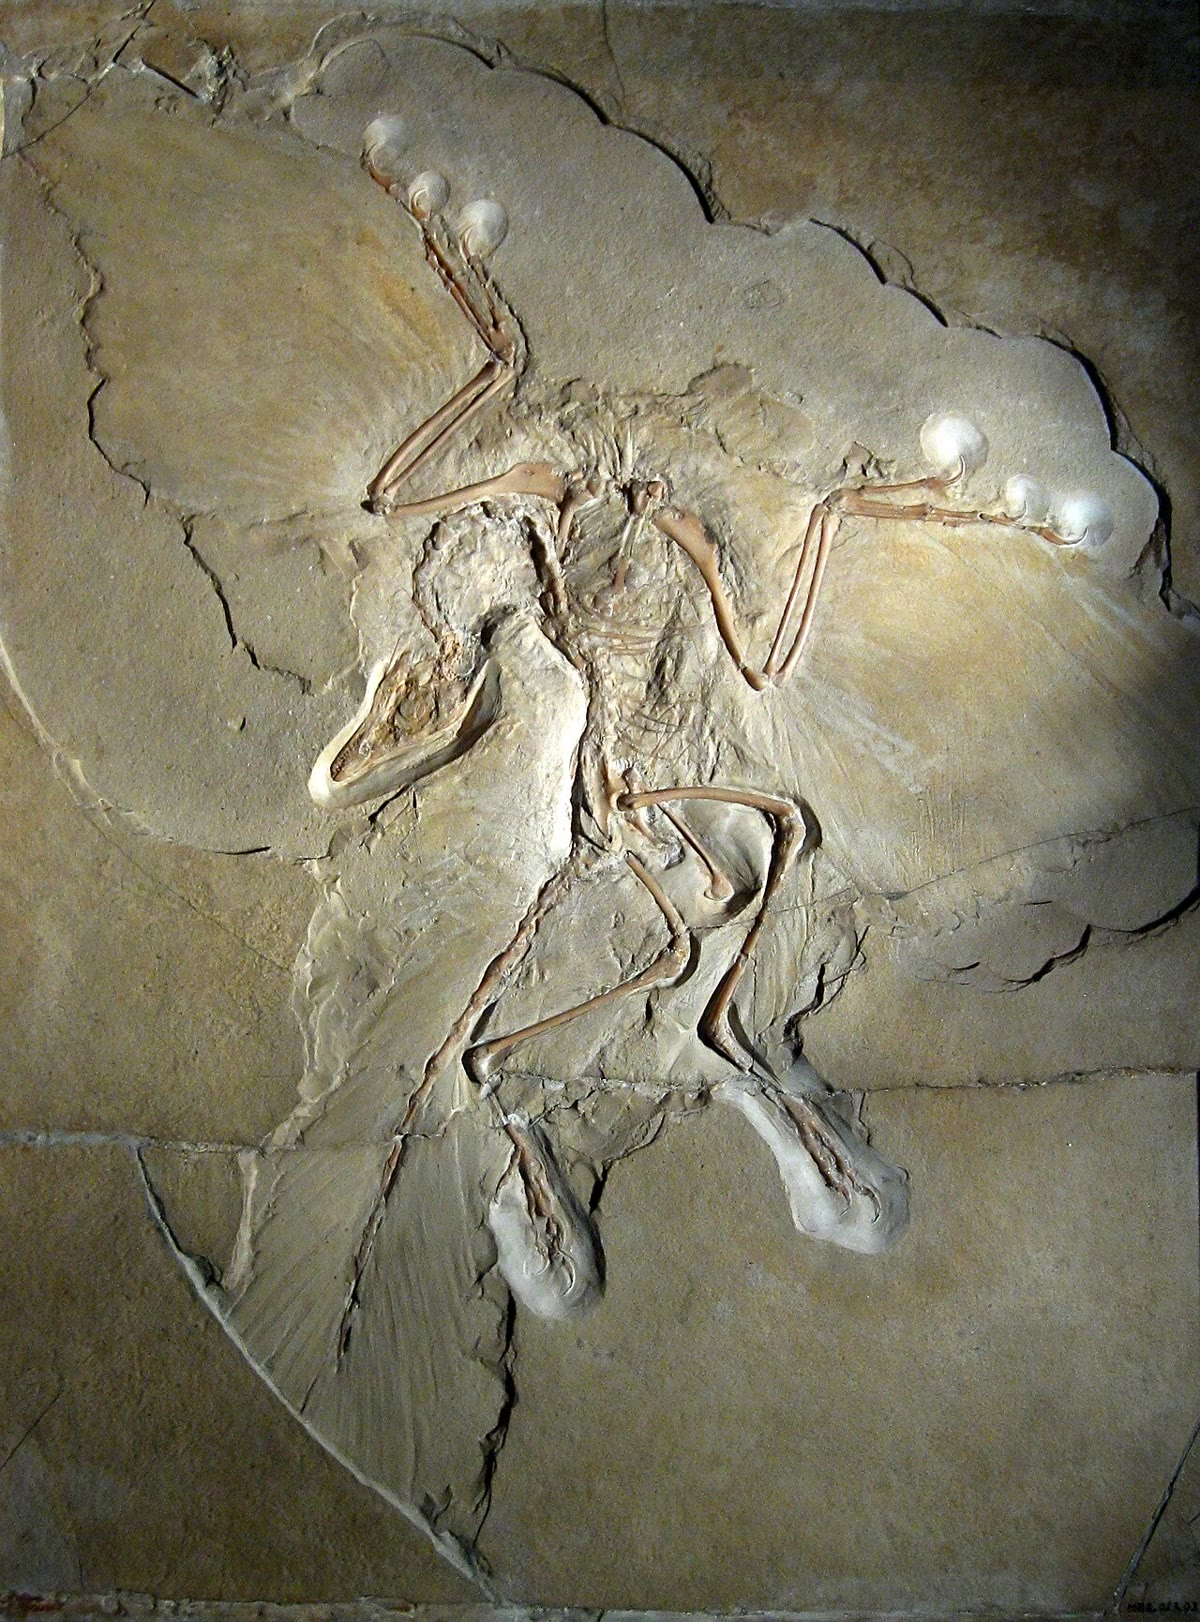
\includegraphics[width=0.5\linewidth]{images/book4/b2-20-archaeopteryx-berlin.jpg}
\par\smallskip{\small सोल्नहोफ़ेन चूना-पत्थरों से \emph{आर्कियोप्टेरिक्स} का बर्लिन नमूना:
हड्डियाँ और पंखों तथा पूँछ के परों की छापें। (H.~Raab, CC~BY-SA~3.0,
विकिमीडिया कॉमन्स के माध्यम से।)}
\end{omfigure}
% ledger: rauhut18:archaeopteryx, gerschermann21:solnhofen

\subsection*{घड़ियों के रूप में जीवाश्म}

पुस्तक 3 ने जैव-क्षेत्र बनाया, यानी अपने जीवाश्मों से परिभाषित स्तरों का एक पिंड, और वह सूचक
जीवाश्म जो उसे पहचानता है। वे कितनी बारीक घड़ी बनाते हैं? एक जुरैसिक अमोनाइट क्षेत्र
लगभग दस लाख वर्ष चल सकता है: सबसे आरंभिक टोआर्सियन क्षेत्र, जिसकी आयु अर्जेंटीना में राख-परतों की
यूरेनियम--सीसा आयुओं से निकाली गई है, 183.73 से \qty{182.77}{Ma} तक फैला है। क्षेत्रों को क्षितिजों में बाँटा जाता है, और उत्तर
जुरैसिक में एक अमोनाइट क्षितिज औसतन \qty{165}{kyr} चलता है।
\emph{आर्कियोप्टेरिक्स} के सभी कंकाल एक ही क्षेत्र से आते हैं जिसमें पाँच क्षितिज हैं, इसलिए यह पक्षी
कोई 0.7 से 1 मिलियन वर्षों में ज्ञात है। पर जीवाश्म केवल एक क्रम देते हैं; वर्षों में आयुएँ
यूरेनियम और सीसे से दिनांकित राख-परतों से, और अवसादी चक्रों से आती हैं। वही राख-परतें टोआर्सियन का आधार $183.73$ पर रखती हैं, अनिश्चितता
$+0.35$ और \qty{-0.50}{Myr} के साथ, जहाँ अंतर्राष्ट्रीय चार्ट \qty{184.2}{Ma} देता है।
% ledger: alsuwaidi22:toarcian, rauhut18:archaeopteryx, ics4:jurassic-stages

\section{पर्यावरण के साक्षी के रूप में जीवाश्म}\label{sec:b2:palaeoenvironments:environment}

किसी जीवाश्म में पर्यावरण पढ़ने के लिए भूविज्ञानी मानता है कि जीव वहीं रहता था जहाँ उसके जीवित
संबंधी रहते हैं, और कि जो प्रक्रियाएँ आज अवसाद पर कार्य करती हैं वे तब भी उसी तरह कार्य करती थीं।

\begin{definition}[वर्तमानवाद]\label{def:b2:palaeoenvironments:actualism}
\emph{वर्तमानवाद}\index{वर्तमानवाद} बीते भूवैज्ञानिक अभिलेखों की उन प्रक्रियाओं, और जीवों
तथा उनके पर्यावरण के उन संबंधों, के द्वारा व्याख्या करने की विधि है जिन्हें आज देखा जा सकता है।
\end{definition}

1830 में चार्ल्स लायल ने अपनी पुस्तक \emph{भूविज्ञान के सिद्धांत} के पहले खंड को यह उपशीर्षक दिया: ``अब
सक्रिय कारणों के संदर्भ से पृथ्वी की सतह के पूर्व परिवर्तनों को समझाने का एक
प्रयास''। इस विधि की सीमाएँ हैं। अनेक समूह विलुप्त हैं, और उनके जीवन-ढंग का
अनुमान उनके आकार और उनके आसपास के अवसाद से लगाना पड़ता है; और अतीत के किसी पर्यावरण का
आज कोई ठीक समरूप न भी हो।
% ledger: lyell1830:title

\begin{definition}[पुरापर्यावरण]\label{def:b2:palaeoenvironments:palaeoenvironment}
\emph{पुरापर्यावरण}\index{पुरापर्यावरण} भौतिक, रासायनिक और
जैविक परिस्थितियों का वह समुच्चय है जो किसी चट्टान के बनने के स्थान और समय पर विद्यमान था: परिवेश, जल की गहराई और
ऊर्जा, उसकी लवणता, तापमान और ऑक्सीजन, तल की प्रकृति, और उस पर का
जीवन।
\end{definition}

\subsection*{जीवाश्म कहाँ रहता था?}

पहला प्रश्न यह है कि क्या जीवाश्म वहीं रहते थे जहाँ वे पड़े हैं।

\begin{definition}[जीवन और मृत्यु समुच्चय; स्वस्थानिक और परस्थानिक जीवाश्म]\label{def:b2:palaeoenvironments:assemblages}
एक \emph{जीवन-समुच्चय}\index{जीवन-समुच्चय} उन जीवों के जीवाश्मों का समूह है जो
साथ रहते थे, जहाँ और जैसे वे रहते थे वैसे ही परिरक्षित; एक \emph{मृत्यु-समुच्चय}\index{मृत्यु-समुच्चय}
मृत्यु के बाद एकत्र हुए अवशेषों का समूह है, जिसमें भिन्न स्थानों और
भिन्न समयों के जीव मिले हो सकते हैं। एक जीवाश्म \emph{स्वस्थानिक}\index{स्वस्थानिक जीवाश्म} है यदि वह
वहीं परिरक्षित है जहाँ जीव रहता था, और \emph{परस्थानिक}\index{परस्थानिक जीवाश्म} यदि वह
दफ़न से पहले कहीं और से लाया गया।
\end{definition}

सुराग परिवहन के हैं। अभी भी बंद सीपियाँ, अपनी वृद्धि-स्थिति में कोई प्रवाल या बिल खोदने वाला द्विकपाटी,
अक्षत नाज़ुक काँटे, किसी समष्टि की सभी आयुएँ उपस्थित: जीवाश्म
संभवतः \omterm{def:b2:palaeoenvironments:assemblages}{स्वस्थानिक} हैं। आकार के अनुसार छँटे अकेले कपाट, घिसे और टूटे खंड, किसी क्रमित परत के आधार पर
सांद्रित सीपियाँ: वे बहाकर लाए गए। सीपियों का कोई \omterm{def:b2:palaeoenvironments:assemblages}{मृत्यु-समुच्चय}, जैसे
ऊपर के तटीय तल पर वाला, अब भी समुदाय का अधिकांश भाग रखता है, पर उसके अनेक वर्षों को
एक परत में समेट देता है: उसके जीवाश्म समय पर औसतित होते हैं।
% ledger: tyler25:live-dead

\subsection*{लवणता और ऑक्सीजन}

कुछ जंतु केवल खुले समुद्र की लवणता सहते हैं: उन्हें स्टेनोहेलाइन (संकीर्ण-लवणसह) कहते हैं। शूलचर्मी,
शीर्षपाद, प्रवाल और, पैलियोज़ोइक में, ट्राइलोबाइट विशिष्ट स्टेनोहेलाइन समूह हैं; उनकी
उपस्थिति सामान्य समुद्री जल के पक्ष में बोलती है, और किसी समृद्ध जीवजात से उनकी अनुपस्थिति उसके विरुद्ध बोल सकती है।
वियतनाम में एक सिल्यूरियन ज्वारनदमुख के निक्षेपों में पादप-मलबा, मछलियों की हड्डियाँ, द्विकपाटी, उदरपाद
और ऑस्ट्राकोड हैं, पर इन समूहों में से कोई नहीं। शूलचर्मी चेंगजियांग जीवसमूह से भी अनुपस्थित हैं,
जो लगभग 518 मिलियन वर्ष पुराना एक \omterm{def:b2:palaeoenvironments:lagerstatte}{लागरश्टेटे} है, यद्यपि वे कैम्ब्रियन के खुले-समुद्री लागरश्टेटेन में
मिलते हैं: चेंगजियांग के जंतु एक डेल्टा के सामने रहते थे, जहाँ मीठा जल लवणता को घटाता-बढ़ाता था।
% ledger: mcgairy21:stenohaline, saleh22:echinoderms, saleh22:age

ऑक्सीजन बिल खोदने वालों के माध्यम से अपना चिह्न छोड़ती है। जहाँ तल के जल में ऑक्सीजन है, जंतु
अवसाद को मिलाते हैं और उसके बारीक पटलन को नष्ट करते हैं; जहाँ वह नहीं है, पटल बचे रहते हैं, बिल
अनुपस्थित होते हैं और पायराइट बनता है, जैसे \cref{ch:b2:phanerozoic-earth} की महासागरीय अनॉक्सी घटनाओं
के काले शेलों में। बिल खोदने वालों के इसी अभाव ने बर्जेस शेल के
शवों की रक्षा की।
% ledger: mussini25:burgess

\subsection*{इक्नोफ़ेसीज़}

\omterm{def:b2:palaeoenvironments:fossil-kinds}{चिह्न जीवाश्म} तल के सबसे अच्छे साक्षी हैं, क्योंकि वे खिसकाए नहीं गए। उनके निर्माता
जल की ऊर्जा, तल की दृढ़ता, भोजन और ऑक्सीजन पर प्रतिक्रिया करते हैं, और
चिह्नों के वही संयोजन पूरे फ़ैनेरोज़ोइक में दोहराए जाते हैं।

\begin{definition}[इक्नोफ़ेसीज़]\label{def:b2:palaeoenvironments:ichnofacies}
एक \emph{इक्नोफ़ेसीज़}\index{इक्नोफ़ेसीज़} \omterm{def:b2:palaeoenvironments:fossil-kinds}{चिह्न जीवाश्मों} का एक आवर्ती संयोजन है जो
पर्यावरणीय परिस्थितियों के एक समुच्चय को दर्शाता है; उसका नाम किसी विशिष्ट चिह्न पर रखा जाता है।
\end{definition}

तट से गहरी द्रोणी तक, किसी समुद्री परिच्छेदिका के अनुदिश चार समुद्री \omterm{def:b2:palaeoenvironments:ichnofacies}{इक्नोफ़ेसीज़} एक के बाद एक
आती हैं (नीचे का चित्र)। \emph{स्कोलिथोस} \omterm{def:b2:palaeoenvironments:ichnofacies}{इक्नोफ़ेसीज़}, जिसमें निलंबन-भक्षियों के ऊर्ध्वाधर, बेलनाकार या
U-आकार के आवास-बिल प्रधान हैं और क्षैतिज चिह्न थोड़े हैं, अग्रतट और तटमुख की
विशिष्ट है। \emph{क्रूज़ियाना} \omterm{def:b2:palaeoenvironments:ichnofacies}{इक्नोफ़ेसीज़}, जिसमें निक्षेप-भक्षियों के बिल प्रधान हैं,
चरने वालों, मांसाहारियों और निलंबन-भक्षियों के चिह्नों के साथ, अपतट की विशिष्ट है:
वह तल जो सामान्य-मौसम तरंग-आधार, यानी वह गहराई जिसके ऊपर साधारण लहरें अवसाद को हिलाती हैं,
और तूफ़ान तरंग-आधार के बीच है, जहाँ केवल तूफ़ानी लहरें पहुँचती हैं। \emph{ज़ूफ़ाइकोस}
\omterm{def:b2:palaeoenvironments:ichnofacies}{इक्नोफ़ेसीज़}, जिसका नाम उस बिल पर है जो अवसाद को एक केंद्रीय अक्ष के चारों ओर सर्पिल चादरों में
उलटता-पलटता है, तूफ़ान तरंग-आधार से नीचे के मग्नतट और ढलान की विशिष्ट है। \emph{नेरेइटीज़}
\omterm{def:b2:palaeoenvironments:ichnofacies}{इक्नोफ़ेसीज़}, अपने नियमित सर्पिल-घुमावदार, कुंडलित और जालीदार बिलों के साथ, जिन्हें कम भोजन पाने वाले जंतुओं
के फंदे और बगीचे माना जाता है, मग्नतट-भंग से परे गहरे समुद्र की विशिष्ट है।
खारे-मीठे जल की खाड़ियों और ज्वारनदमुखों में कुछ ही प्रजातियों वाली एक क्रूज़ियाना \omterm{def:b2:palaeoenvironments:ichnofacies}{इक्नोफ़ेसीज़} नियम है।
% ledger: buatois20:ichnofacies, miguez21:ichnofacies, zhang15:zoophycos, buatois25:graphoglyptids, paz23:nereites

\begin{omfigure}
\centering
\begin{tikzpicture}[font=\scriptsize, x=1cm, y=1cm]
% sea and floor (schematic, not to scale)
\fill[omSea!20] (0.6,0) -- (14,0) -- (14,-3.6) -- (11.2,-3.6) -- (9.6,-1.9) -- (6.2,-1.5)
  -- (3.2,-0.9) -- (1.2,-0.15) -- cycle;
\fill[omLithSand!45] (0,0.25) -- (0.6,0) -- (1.2,-0.15) -- (3.2,-0.9) -- (6.2,-1.5)
  -- (9.6,-1.9) -- (11.2,-3.6) -- (14,-3.6) -- (14,-4.3) -- (0,-4.3) -- cycle;
\draw[black!70, line width=0.6pt] (0,0.25) -- (0.6,0) -- (1.2,-0.15) -- (3.2,-0.9) -- (6.2,-1.5)
  -- (9.6,-1.9) -- (11.2,-3.6) -- (14,-3.6);
\draw[omSea!80!black, line width=0.6pt] (0.6,0) -- (14,0);
\node[anchor=south east, omSea!80!black] at (14,0) {समुद्र-स्तर};
% wave bases
\draw[dashed, black!60] (2.133,-0.5) -- (14,-0.5) node[anchor=south east, black!70] {सामान्य-मौसम तरंग-आधार};
\draw[dashed, black!60] (4.7,-1.2) -- (14,-1.2) node[anchor=south east, black!70] {तूफ़ान तरंग-आधार};
% zone labels
\node[align=center] at (1.9,0.55) {अग्रतट,\\तटमुख};
\node[align=center] at (4.6,0.55) {अपतट};
\node[align=center] at (8.0,0.55) {मग्नतट};
\node[align=center] at (10.5,0.55) {ढलान};
\node[align=center] at (12.7,0.55) {द्रोणी};
% Skolithos: vertical tubes
\foreach \x in {1.75,1.95,2.15,2.35} {\draw[black!80, line width=0.7pt] (\x,{-0.15-0.375*(\x-1.2)}) -- ++(0,-0.55);}
\node[align=center] at (2.1,-2.15) {\textbf{\emph{स्कोलिथोस}}\\ऊर्ध्वाधर नलिकाएँ};
% Cruziana: horizontal bilobed trails
\foreach \x in {4.0,4.8} {\draw[black!80, line width=0.6pt] (\x,-1.45) .. controls ++(0.2,0.08) .. ++(0.5,0);
  \draw[black!80, line width=0.6pt] (\x,-1.53) .. controls ++(0.2,-0.08) .. ++(0.5,0);}
\node[align=center] at (4.7,-2.35) {\textbf{\emph{क्रूज़ियाना}}\\भोजन-बिल,\\चरने के चिह्न};
% Zoophycos: spreite arcs
\foreach \r in {0.12,0.22,0.32} {\draw[black!80, line width=0.5pt] (8.0,-2.25) ++(-\r,0) arc (180:360:\r cm and 0.5*\r cm);}
\draw[black!80, line width=0.6pt] (8.0,-2.25) -- (8.0,-1.8);
\node[align=center] at (8.0,-3.05) {\textbf{\emph{ज़ूफ़ाइकोस}}\\सर्पिल\\चादरें};
% Nereites: meander
\draw[black!80, line width=0.6pt, domain=0:2.2, samples=80, smooth] plot (12.0+\x*0.5,{-3.9+0.12*sin(\x*720)});
\node[align=center, anchor=north] at (12.5,-4.35) {\textbf{\emph{नेरेइटीज़}}\\घुमाव, जाल};
\end{tikzpicture}
\par\smallskip{\small ज़ाइलाकर के मॉडल की चार समुद्री \omterm{def:b2:palaeoenvironments:ichnofacies}{इक्नोफ़ेसीज़}, तट से गहरी द्रोणी तक की एक परिच्छेदिका के
अनुदिश, हर एक के एक विशिष्ट चिह्न के रेखाचित्र के साथ; गहराइयाँ पैमाने पर नहीं हैं।
चिह्न गहराई से अधिक ऊर्जा, भोजन और ऑक्सीजन पर प्रतिक्रिया करते हैं।}
\end{omfigure}
% ledger: buatois20:ichnofacies, miguez21:ichnofacies, zhang15:zoophycos, buatois25:graphoglyptids, paz23:nereites

गहराई सीधे कार्य नहीं करती। किसी गहरे-समुद्री वाहिका में, जहाँ गंदलाव-धाराएँ प्रबल हैं, स्कोलिथोस
\omterm{def:b2:palaeoenvironments:ichnofacies}{इक्नोफ़ेसीज़} के ऊर्ध्वाधर बिल किसी भी तरंग-आधार से बहुत नीचे दिखते हैं; और किसी डेल्टा के पास, जहाँ मीठा
जल और कीचड़ उमड़कर आते हैं, अपतट के चिह्न अन्यत्र से निर्धन होते हैं। निर्माता भी
समय के साथ खिसके: बिल \emph{ज़ूफ़ाइकोस} पैलियोज़ोइक में मग्नतट पर रहता था, मेसोज़ोइक में निचले मग्नतट
और ढलान पर, और सीनोज़ोइक में गहरे समुद्र में। एक \omterm{def:b2:palaeoenvironments:ichnofacies}{इक्नोफ़ेसीज़} तल की
परिस्थितियाँ दर्ज करती है, जिनसे गहराई का केवल अनुमान लगाया जाता है, और उस अनुमान में
चट्टान की आयु का उपयोग करना होता है।
% ledger: buatois20:ichnofacies, zhang15:zoophycos

\begin{inthefield}[परत-दर-परत जीवाश्म गिनना]
किसी खंड से पर्यावरण का पुनर्निर्माण करने वाली पुराजीवविज्ञानी हर परत को उसकी
शैलिकी, मोटाई और अवसादी संरचनाओं के साथ लॉग करती है, और फिर उसके जीवाश्म: कौन-से समूह, कितने,
सीपियाँ पूरी हैं या टूटी, बंद या खुली, छँटी या नहीं, और वे किस स्थिति में पड़ी हैं।
\omterm{def:b2:palaeoenvironments:fossil-kinds}{चिह्न जीवाश्म} वहाँ दर्ज किए जाते हैं जहाँ वे दिखते हैं, संस्तरण-तलों पर और ऊर्ध्वाधर फलकों में,
उस गहराई के साथ जहाँ तक बिल पहुँचते हैं। क्योंकि सीपी खिसकाई जा सकती है पर बिल नहीं,
दोनों सूचियाँ अलग रखी जाती हैं; पर्यावरण पहले चिह्नों से पढ़ा जाता है, और \omterm{def:b2:palaeoenvironments:fossil-kinds}{काय जीवाश्मों}
को फिर परिवहन के संकेतों के लिए जाँचा जाता है।
\end{inthefield}

\begin{omfigure}
\centering
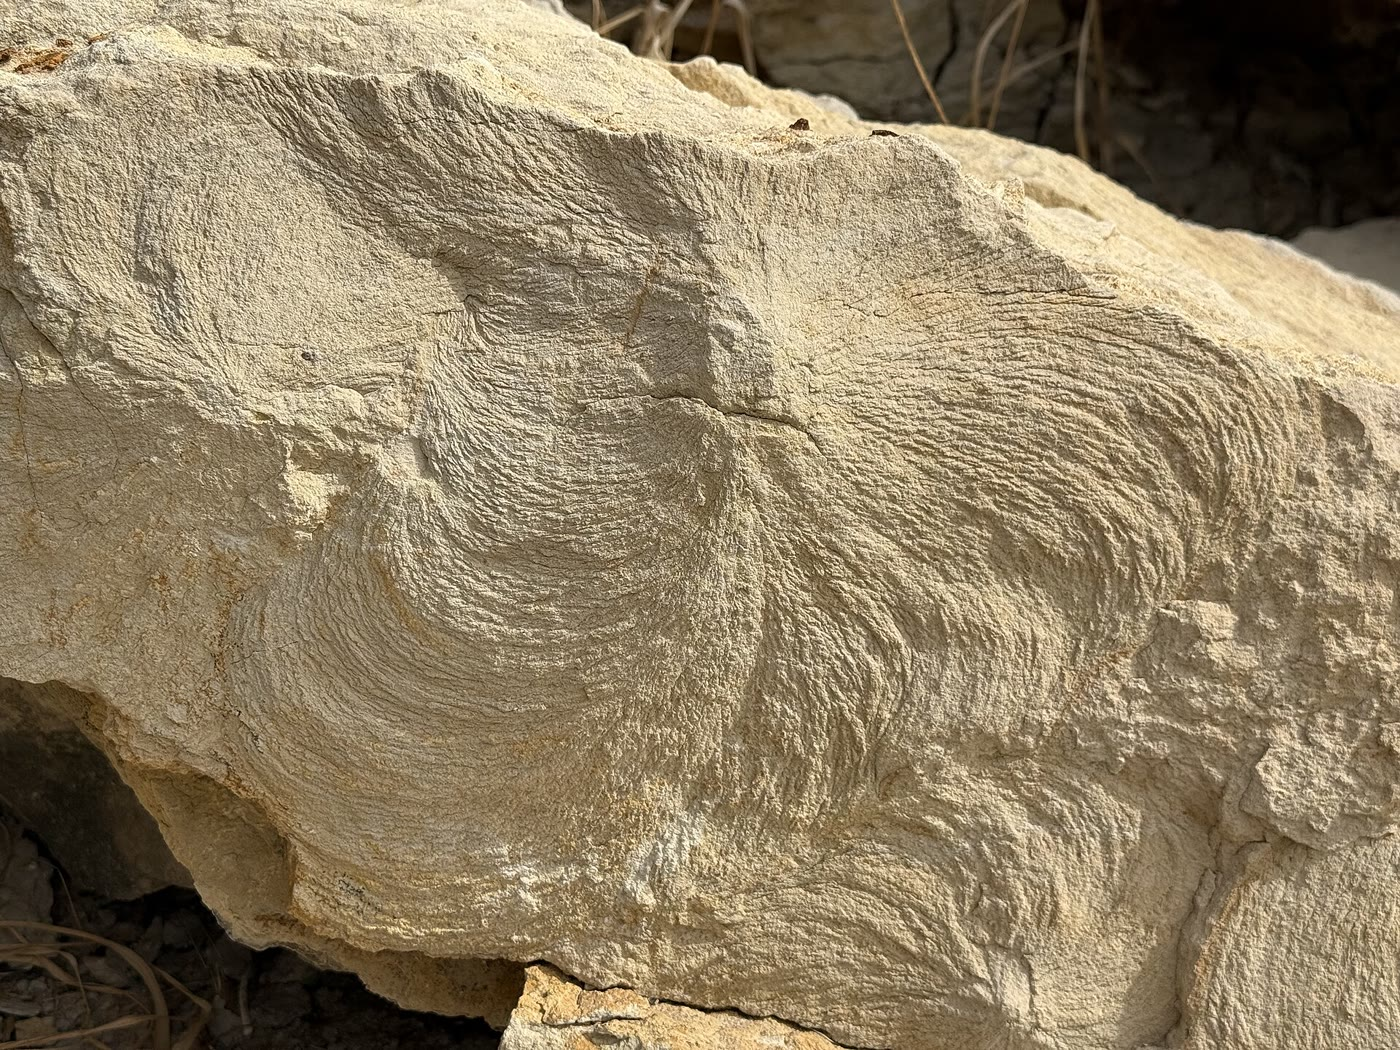
\includegraphics[width=0.5\linewidth]{images/book4/b2-20-zoophycos.jpg}
\par\smallskip{\small साग्रेस, पुर्तगाल में एक खंड पर \emph{ज़ूफ़ाइकोस}: चाप उलटे-पलटे अवसाद की
एक सर्पिल चादर की पटलिकाएँ हैं। (Amada44, CC~BY~4.0, विकिमीडिया कॉमन्स के माध्यम से।)}
\end{omfigure}
% ledger: zhang15:zoophycos

\section{एक लुप्त समुद्र को पढ़ना}\label{sec:b2:palaeoenvironments:varden}

पर्यावरण एक-दूसरे के बगल में होते हैं: एक समुद्र-तट, एक अपतट तल, एक गहरा मग्नतट। जब समुद्र उठता है या
तल धँसता है, तो हर पर्यावरण अपने पड़ोसी के ऊपर भूमि की ओर खिसकता है, और उसके निक्षेप
पड़ोसी के निक्षेपों के ऊपर आ जाते हैं। फ़ेसीज़ का एक ऊर्ध्वाधर अनुक्रम, बिना किसी विराम के, इस प्रकार
उन पर्यावरणों का क्रम दोहराता है जो एक-दूसरे के बगल में थे; पुस्तक 5 इस नियम,
वाल्टर के नियम, को अपना प्रारंभ-बिंदु बनाती है। नीचे से ऊपर पढ़ा गया लॉग एक स्थान के आर-पार
खिसकते तट की फ़िल्म है।

वार्डन पहाड़ियों का आवरण, शृंखला का कल्पित क्षेत्र, एक पूर्ण उदाहरण बनाता है। उसकी
मोटाइयाँ क्षेत्र के मॉडल की हैं; नीचे के चित्र के जीवाश्म उसके लिए कल्पित हैं,
पर हर एक ऐसा चुना गया है जिसे उस प्रकार की वास्तविक चट्टानें रख सकती हैं। चूना-पत्थर को
टोआर्सियन दिया गया है, 184.2 से \qty{174.7}{Ma} तक, और शेल को आलेनियन से कैलोवियन तक,
\qty{174.7}{Ma} से \qty{161.5}{Ma} तक।
% ledger: data:b4-palaeoenv, ics4:jurassic-stages

\begin{omfigure}
\centering
% figdata/bachelor-2/palaeoenv.py part log (thicknesses from figdata/shared/region.py)
\begin{tikzpicture}[x=1cm, y=0.0165cm, font=\scriptsize]
% scale
\draw[black!70] (-0.35,0) -- (-0.35,460);
\foreach \z in {0,100,...,400} {\draw[black!70] (-0.45,\z) -- (-0.35,\z) node[left=3pt] {\z};}
\node[rotate=90, anchor=south] at (-1.15,230) {आवरण के आधार से ऊँचाई (m)};
% units
\fill[lith sandstone] (0,0) rectangle (2.2,120);
\fill[lith limestone] (0,120) rectangle (2.0,180);
\fill[lith limestone] (0,180) rectangle (1.6,300);
\fill[lith shale] (0,300) rectangle (1.1,400);
\fill[om lith={icsCretaceous!35}{om limestone}] (0,400) -- (1.4,400) -- (1.4,452)
  .. controls (1.0,466) and (0.6,446) .. (0.3,458) -- (0,455) -- cycle;
\draw[black!70] (0,0) rectangle (2.2,120);
\draw[black!70] (0,120) rectangle (2.0,180);
\draw[black!70] (0,180) rectangle (1.6,300);
\draw[black!70] (0,300) rectangle (1.1,400);
\draw[black!70] (0,400) -- (1.4,400) -- (1.4,452) .. controls (1.0,466) and (0.6,446) ..
  (0.3,458) -- (0,455) -- cycle;
\node[anchor=west, font=\tiny] at (1.45,460) {अपरदित शीर्ष};
% unit names
\node[anchor=west, align=left] at (2.6,60) {\textbf{बलुआ पत्थर}, \qty{120}{m}\\ट्राइऐसिक};
\node[anchor=west, align=left] at (2.6,150) {\textbf{ऊलाइटी चूना-पत्थर}, \qty{60}{m}\\टोआर्सियन};
\node[anchor=west, align=left] at (2.6,240) {\textbf{महीन चूना-पत्थर}, \qty{120}{m}\\टोआर्सियन};
\node[anchor=west, align=left] at (2.6,350) {\textbf{शेल}, \qty{100}{m}\\आलेनियन--कैलोवियन};
\node[anchor=west, align=left] at (2.6,424) {\textbf{खड़िया}\\क्रिटेशियस};
% content
\node[anchor=west, align=left, text width=6.9cm] at (6.3,60) {अपरदित आधारों पर तिर्यक-परतदार वाहिका-भराव;
  जड़ों के चिह्न; पादप-खंड; कोई समुद्री जीवाश्म नहीं};
\node[anchor=west, align=left, text width=6.9cm] at (6.3,150) {तिर्यक-परतदार ऊइड; ऊर्ध्वाधर नलिकाएँ
  और U-आकार के बिल; घिसे सीपी-खंड};
\node[anchor=west, align=left, text width=6.9cm] at (6.3,240) {क्रिनॉइड अस्थिकाएँ, ब्रैकियोपॉड,
  बेलेम्नाइट, अमोनाइट; रेंगने की लकीरें और भोजन-बिल; तीखे आधारों वाली टूटी सीपियों
  की परतें};
\node[anchor=west, align=left, text width=6.9cm] at (6.3,350) {गहरा धूसर, कहीं-कहीं पटलित;
  पायराइट; अमोनाइट और पतली सीपी वाले द्विकपाटी; हल्की परतों में सर्पिल स्प्राइटे बिल};
\node[anchor=west, align=left, text width=6.9cm] at (6.3,424) {कोकोलिथ; समुद्री अर्चिन, स्पंज;
  चकमक गुलिकाएँ; सर्वत्र बिलयुक्त};
\foreach \z in {120,180,300,400} {\draw[black!25] (2.25,\z) -- (13.2,\z);}
\node[font=\scriptsize\bfseries, anchor=south west] at (2.6,462) {इकाई और आयु};
\node[font=\scriptsize\bfseries, anchor=south west] at (6.3,462) {परतों में क्या है};
\end{tikzpicture}
\par\smallskip{\small वार्डन पहाड़ियों का आवरण एक लॉग के रूप में, उसकी इकाइयों की सामग्री के साथ।
मोटाइयाँ क्षेत्र के मॉडल की हैं, खड़िया को छोड़कर, जिसका अपरदित शीर्ष यहाँ छोटा काट दिया गया है
(\cref{ex:b2:palaeoenvironments:shale} की अभिनति में \qty{766}{m} मोटी); स्तंभ की चौड़ाई कण-आकार के साथ बढ़ती है;
जीवाश्म और उनकी आयुएँ क्षेत्र के लिए कल्पित हैं।}
\end{omfigure}
% ledger: data:b4-palaeoenv, ics4:jurassic-stages

\begin{example}[वार्डन आवरण का आधार]\label{ex:b2:palaeoenvironments:base}
बलुआ पत्थर में अपरदित आधारों पर वाहिका-भराव, जड़ें और पादप-खंड हैं, और कोई समुद्री
जीवाश्म नहीं: वह भूमि पर नदियों द्वारा जमाया गया। ऊपर के ऊलाइटी चूना-पत्थर में तिर्यक-परतदार ऊइड हैं,
जो विक्षुब्ध जल में लुढ़कते हुए बढ़ते हैं, स्कोलिथोस \omterm{def:b2:palaeoenvironments:ichnofacies}{इक्नोफ़ेसीज़} की ऊर्ध्वाधर नलिकाएँ और U-आकार के बिल हैं,
और घिसे सीपी-खंड, सभी \omterm{def:b2:palaeoenvironments:assemblages}{परस्थानिक}: तटमुख का एक उथला टीला,
लहरों से बुहारा हुआ। दोनों के बीच समुद्र आ पहुँचा: संपर्क एक \omterm{def:b2:phanerozoic-earth:transgression}{समुद्री ट्रांसग्रेशन} दर्ज करता है।
वाल्टर के नियम के क्रम में, नदी-मैदान के बाद तट आया, फिर उथला टीला।
\end{example}
% ledger: buatois20:ichnofacies

\subsection*{समुद्र-तल कितनी तेज़ी से भरा?}

एक जैव-क्षेत्र एक अवधि देता है, एक लॉग एक मोटाई देता है, और उनका अनुपात एक दर है। पर
अवसाद के जमने के बाद से मोटाई सिकुड़ गई है: छिद्रों का जल बाहर निचोड़ा जा चुका है,
और केवल कण संरक्षित रहते हैं।

\begin{proposition}[संपीड़ित परत की संचयन-दर]\label{prop:b2:palaeoenvironments:rate}
वर्तमान मोटाई $h$ और माध्य छिद्रता $\varphi$ वाली एक परत, जो समय $\Delta t$ में
छिद्रता $\varphi_0$ के साथ जमी, इस दर से संचित हुई
\[
  r = \frac{h\,(1 - \varphi)}{(1 - \varphi_0)\,\Delta t}
\]
ताज़ा अवसाद की, और कणों की दर $h(1-\varphi)/\Delta t$ से, जो
$\varphi_0$ पर निर्भर नहीं करती।
\end{proposition}

\begin{proof}
प्रति इकाई क्षेत्रफल, परत कणों का आयतन $h(1 - \varphi)$ रखती है, जो पुस्तक 3 की ठोस मोटाई
है। संपीड़न जल को बाहर निकालता है पर कण न जोड़ता है न हटाता है, इसलिए ताज़ा
अवसाद, छिद्रता $\varphi_0$ का, मोटाई $h_0$ रखता था, जहाँ $h_0(1 - \varphi_0) = h(1 -
\varphi)$। $h_0$ और ठोस मोटाई को $\Delta t$ से भाग देने पर दोनों दरें मिलती हैं।
\end{proof}

जब छिद्रता मापी नहीं गई, तब एथी का नियम उसे गहराई से देता है। नीचे का चित्र
चार शैलिकियों के लिए यह नियम दिखाता है, और वह गुणक $(1 - \varphi(z))/(1 - \varphi_0)$ जिससे अब गहराई $z$ पर स्थित किसी पतली
परत को खींचना होगा ताकि सतह पर उसकी मोटाई मिले। खड़िया और शेल
बहुत जल के साथ आरंभ करते हैं और उसे तेज़ी से खोते हैं: \qty{1000}{m} पर शेल की एक पतली परत जमते समय 1.68 गुना
मोटी थी, खड़िया की एक परत 2.19 गुना।
% ledger: pybacktrack:compaction, pybacktrack4:limestone, data:b4-palaeoenv

\begin{omfigure}
\centering
% figdata/bachelor-2/palaeoenv.py parts poro and ratio
\begin{tikzpicture}
\begin{groupplot}[group style={group size=2 by 1, horizontal sep=1.6cm},
  width=0.46\linewidth, height=6.2cm, y dir=reverse, ymin=0, ymax=3000,
  tick label style={font=\scriptsize}, label style={font=\small}, xtick pos=bottom,
  ytick pos=left, scaled y ticks=false, yticklabel style={/pgf/number format/1000 sep={\,}}]
\nextgroupplot[xmin=0, xmax=0.75, xlabel={छिद्रता $\varphi$}, ylabel={गहराई $z$ (\unit{m})},
  legend style={at={(0.5,1.04)}, anchor=south, draw=none, font=\scriptsize, legend columns=2}]
\addplot[omThm, line width=1pt] table[x=shale, y=z_m] {figdata/out/bachelor-2-palaeoenv-poro.dat};
\addlegendentry{शेल}
\addplot[omSea!80!black, line width=1pt, dashed] table[x=sandstone, y=z_m] {figdata/out/bachelor-2-palaeoenv-poro.dat};
\addlegendentry{बलुआ पत्थर}
\addplot[black, line width=1pt, dotted] table[x=chalk, y=z_m] {figdata/out/bachelor-2-palaeoenv-poro.dat};
\addlegendentry{खड़िया}
\addplot[green!45!black, line width=1pt, dash dot] table[x=limestone, y=z_m] {figdata/out/bachelor-2-palaeoenv-poro.dat};
\addlegendentry{चूना-पत्थर}
\nextgroupplot[xmin=1, xmax=3.2, xlabel={पुनर्स्थापन गुणक $(1-\varphi)/(1-\varphi_0)$}]
\addplot[omThm, line width=1pt] table[x=shale, y=z_m] {figdata/out/bachelor-2-palaeoenv-ratio.dat};
\addplot[omSea!80!black, line width=1pt, dashed] table[x=sandstone, y=z_m] {figdata/out/bachelor-2-palaeoenv-ratio.dat};
\addplot[black, line width=1pt, dotted] table[x=chalk, y=z_m] {figdata/out/bachelor-2-palaeoenv-ratio.dat};
\addplot[green!45!black, line width=1pt, dash dot] table[x=limestone, y=z_m] {figdata/out/bachelor-2-palaeoenv-ratio.dat};
\end{groupplot}
\end{tikzpicture}
\par\smallskip{\small बायाँ: एथी के नियम से गहराई के विरुद्ध छिद्रता, शेल, बलुआ पत्थर और खड़िया के लिए स्क्लेटर
और क्रिस्टी (1980) के स्थिरांकों और चूना-पत्थर के लिए ट्यूरर और मेनार्ड (2003) के स्थिरांकों के साथ,
जैसा पाइबैकट्रैक सॉफ़्टवेयर में सारणीबद्ध है। दायाँ: वह गुणक जिससे गहराई $z$ पर एक पतली परत
सतह पर अपनी मोटाई तक पुनर्स्थापित होती है।}
\end{omfigure}
% ledger: pybacktrack:compaction, pybacktrack4:limestone, data:b4-palaeoenv

\begin{example}[वार्डन शेल]\label{ex:b2:palaeoenvironments:shale}
वार्डन पहाड़ियों की अभिनति में खड़िया \qty{766}{m} मोटी है, इसलिए शेल
766 और \qty{866}{m} के बीच है। शेल के स्थिरांकों, $\varphi_0 = 0.63$ और $\lambda =
\qty{1960}{m}$, के साथ पुस्तक 3 की ठोस मोटाई $100 - 0.63 \times 1960 \times
(e^{-766/1960} - e^{-866/1960}) = \qty{58.4}{m}$ है, यानी माध्य छिद्रता 0.416। उन्हीं कणों के साथ
सतह पर वापस लाने पर परत \qty{148.6}{m} मोटी है। आलेनियन के आधार से कैलोवियन के शीर्ष तक के
\qty{13.2}{Myr} में शेल $100/13.2 =
\qty{7.6}{m}$ प्रति मिलियन वर्ष की दर से संचित हुआ जैसा वह अब है, $148.6/13.2 = \qty{11.3}{m}$ प्रति मिलियन
वर्ष ताज़ी कीचड़ की दर से, और कणों की \qty{4.4}{m} प्रति मिलियन वर्ष की दर से। वर्तमान मोटाई
दर को एक-तिहाई कम बताती है।
\end{example}
% ledger: data:b4-palaeoenv, pybacktrack:compaction, ics4:jurassic-stages

शेल कभी और भी गहरा, अब अपरदित हो चुकी खड़िया के नीचे, रहा हो सकता है; तब सुधार एक
न्यूनतम है। सप्ताहांत समस्या प्रस्ताव को चूना-पत्थर पर लागू करती है, जहाँ छिद्रता
मापी गई थी।

\section*{अभ्यास}\label{sec:b2:palaeoenvironments:exercises}

अभ्यासों के आँकड़े, अन्यथा न कहा जाए तो: एथी का नियम $\varphi = \varphi_0 e^{-z/\lambda}$,
$\varphi_0 = 0.63$, $\lambda = \qty{1960}{m}$ (शेल), $0.49$, \qty{3704}{m} (बलुआ पत्थर),
$0.70$, \qty{1408}{m} (खड़िया), $0.51$, \qty{4545}{m} (चूना-पत्थर) के साथ; कैल्साइट \qty{2710}{kg.m^{-3}},
छिद्र-जल \qty{1000}{kg.m^{-3}}; अंतर्राष्ट्रीय चार्ट की आयुएँ: टोआर्सियन 184.2 से
\qty{174.7}{Ma}।
% ledger: pybacktrack:compaction, pybacktrack4:limestone, ics4:jurassic-stages

\begin{exercise}[$\star$]\label{exo:b2:palaeoenvironments:1}
एक तटीय तल के 51 स्थलों पर अकशेरुकियों की 135 प्रजातियाँ जीवित मिलीं, 150 तल पर मृत
सीपियों और कंकालों में, और 112 ऐसी जिनका जीवाश्म अभिलेख भी है। (क)~तीसरी
संख्या को पहली दोनों में से हर एक के भिन्न के रूप में व्यक्त कीजिए। (ख)~मृत जीवितों से अधिक कैसे हो सकते हैं? (ग)~आप
किन भोजन-समूहों के मृतों में कम प्रतिनिधित्व की अपेक्षा करेंगे, और क्यों?
\end{exercise}
% ledger: tyler25:live-dead, tyler25:soft-bodied

\begin{exercise}[$\star$]\label{exo:b2:palaeoenvironments:2}
एक उत्तर जुरैसिक अमोनाइट क्षितिज औसतन \qty{165}{kyr} चलता है। (क)~पाँच क्षितिज कितना
चलते हैं? \emph{आर्कियोप्टेरिक्स} के लिए दिए गए 0.7 से 1 मिलियन वर्षों से तुलना कीजिए। (ख)~सबसे आरंभिक
टोआर्सियन क्षेत्र 183.73 से \qty{182.77}{Ma} तक फैला है: उसमें औसत लंबाई के कितने क्षितिज समाते?
(ग)~किसी वंशक्रम के विकास का अनुसरण करने के लिए क्षेत्र नहीं, क्षितिज क्यों महत्त्वपूर्ण हैं?
\end{exercise}
% ledger: rauhut18:archaeopteryx, alsuwaidi22:toarcian

\begin{exercise}[$\star$]\label{exo:b2:palaeoenvironments:3}
हर समुच्चय की \omterm{def:b2:palaeoenvironments:ichnofacies}{इक्नोफ़ेसीज़} और परिवेश बताइए। (क)~पतले गंदलाव-निक्षेपों के तलों पर घुमावदार चरने की लकीरें और नियमित
बिल-जाल। (ख)~स्वच्छ, तिर्यक-परतदार रेत में पास-पास ऊर्ध्वाधर नलिकाएँ। (ग)~तूफ़ानी रेतों के बीच गादयुक्त
परतों में निक्षेप-भक्षियों के प्रचुर क्षैतिज बिल और चरने के चिह्न। (घ)~तरंग-लहरिकाओं से रहित एक महीन, गहरी कीचड़ में
सर्पिल स्प्राइटे बिल,
मेसोज़ोइक चट्टानों में।
\end{exercise}
% ledger: buatois20:ichnofacies, paz23:nereites

\begin{exercise}[$\star$]\label{exo:b2:palaeoenvironments:4}
परत A में क्रिनॉइड, ब्रैकियोपॉड, प्रवाल और ट्राइलोबाइट हैं; उसी आयु की परत B में पादप-मलबा,
मछलियों की हड्डियाँ, कुछ द्विकपाटी और उदरपाद, और ऑस्ट्राकोड की केवल दो प्रजातियों के अनेक
व्यष्टि हैं। (क)~हर एक अपने जल की लवणता के बारे में क्या कहता है? (ख)~परत B में
परत A के समूह नहीं हैं: वह अनुपस्थिति एक तर्क क्यों है, जबकि एक परत से एक जीवाश्म की अनुपस्थिति नहीं?
(ग)~कौन-से अन्य प्रेक्षण परत B की व्याख्या को परखेंगे?
\end{exercise}
% ledger: mcgairy21:stenohaline, saleh22:echinoderms

\begin{exercise}[$\star\star$]\label{exo:b2:palaeoenvironments:5}
\cref{ex:b2:palaeoenvironments:shell} की सीपी के साथ \cref{prop:b2:palaeoenvironments:burial}
का उपयोग कीजिए, $k = \qty{0.05}{yr^{-1}}$ और $h = \qty{0.1}{m}$। (क)~वह
अवसादन-दर ज्ञात कीजिए जिस पर आधी सीपियाँ सुरक्षा तक पहुँचती हैं। (ख)~उस मान से दर आधी करने पर $P$ किस
गुणक से बदलता है? (ग)~दुगुनी मोटी सीपी तल पर दुगुने समय तक बचती है।
\qty{1}{mm.yr^{-1}} पर, उसके परिरक्षित होने की संभावना कितनी अधिक है? (घ)~यह किसी जीवाश्म समुच्चय में
पतली और मोटी सीपियों के अनुपात के बारे में क्या संकेत देता है?
\end{exercise}
% ledger: tyler25:soft-bodied

\begin{exercise}[$\star\star$]\label{exo:b2:palaeoenvironments:6}
राख-परतें चाकाय मेलेहुए में टोआर्सियन के आधार को $183.73$, $+0.35$, \qty{-0.50}{Myr} पर दिनांकित करती हैं;
अंतर्राष्ट्रीय चार्ट \qty{184.2}{Ma} देता है। (क)~क्या चार्ट का मान अनिश्चितता के भीतर है?
वह ऊपरी सीमा से कितना चूकता है? (ख)~सबसे आरंभिक टोआर्सियन क्षेत्र
\qty{182.77}{Ma} पर समाप्त होता है: उसकी अवधि ज्ञात कीजिए। (ग)~मान लीजिए यह क्षेत्र किसी खंड में \qty{6}{m} मोटा है:
संचयन की दर क्या है? (घ)~कोई जैव-क्षेत्र समय में हर जगह एक-सा क्यों हो सकता है जबकि उसकी
मोटाई स्थान-स्थान पर भिन्न होती है?
\end{exercise}
% ledger: alsuwaidi22:toarcian, ics4:jurassic-stages

\begin{exercise}[$\star\star$]\label{exo:b2:palaeoenvironments:7}
वार्डन अभिनति में बलुआ पत्थर भूमि से 1046 और \qty{1166}{m} नीचे के बीच है। (क)~एथी के नियम से
शीर्ष पर और आधार पर उसकी छिद्रता ज्ञात कीजिए, और उसकी माध्य छिद्रता, दोनों के औसत से,
तीन दशमलव तक पूर्णांकित। (ख)~उसकी ठोस मोटाई ज्ञात कीजिए। (ग)~माध्य छिद्रता पर पतली-परत गुणक से उसे
सतह पर पुनर्स्थापित कीजिए। (घ)~सटीक पुनर्स्थापन
\qty{147.0}{m} देता है। पतली-परत अनुमान थोड़ा अधिक बड़ा क्यों है?
\end{exercise}
% ledger: data:b4-palaeoenv, pybacktrack:compaction

\begin{exercise}[$\star\star$]\label{exo:b2:palaeoenvironments:8}
एक घनत्व-लॉग वार्डन चूना-पत्थर में \qty{2573}{kg.m^{-3}} पढ़ता है, जो छिद्रों में जल वाले कैल्साइट कणों
से बना है। (क)~दिखाइए कि छिद्रता $\varphi = (\rho_{\text{कण}} -
\rho)/(\rho_{\text{कण}} - \rho_{\text{जल}})$ है और उसकी गणना कीजिए। (ख)~अभिनति में
चूना-पत्थर की मध्य-गहराई, \qty{956}{m}, पर एथी का नियम चूना-पत्थर के स्थिरांकों के साथ क्या बताता है?
(ग)~डायाजेनेसिस की कौन-सी प्रक्रिया अंतर समझा सकती है?
\end{exercise}
% ledger: pybacktrack4:limestone, data:b4-palaeoenv

\begin{exercise}[$\star\star$]\label{exo:b2:palaeoenvironments:9}
जुरैसिक चट्टानों की एक खड़ी चट्टान आधार से ऊपर दिखाती है: नियमित घुमावों और बिल-जालों वाले पतले
गंदलाव-निक्षेप; सर्पिल स्प्राइटे बिलों वाली गहरी कीचड़; तूफ़ानी रेतों के बीच निक्षेप-भक्षी बिलों वाली
गादयुक्त परतें; ऊर्ध्वाधर नलिकाओं वाली
स्वच्छ तिर्यक-परतदार रेत; फिर जड़ों वाला एक कोयला। (क)~हर भाग की व्याख्या कीजिए। (ख)~जल गहरा हुआ या
उथला? (ग)~दो कारण बताइए जो यह अनुक्रम उत्पन्न कर सकते हैं, और बताइए कि उनके बीच निर्णय
किससे होगा। (घ)~पहले भाग से चौथे तक, बाकी के बिना, एक तीखी छलाँग
चेतावनी क्यों है?
\end{exercise}
% ledger: buatois20:ichnofacies, paz23:nereites

\begin{exercise}[$\star\star\star$]\label{exo:b2:palaeoenvironments:10}
एक कोमल-शरीर जंतु तल पर औसतन एक वर्ष बचता है ($k = \qty{1}{yr^{-1}}$), एक
सीपी एक शताब्दी; दोनों $h = \qty{0.1}{m}$ के नीचे सुरक्षित हैं। (क)~1, 10 और \qty{100}{mm.yr^{-1}} पर
उनके परिरक्षण की संभावनाओं की तुलना कीजिए। (ख)~वह दर ज्ञात कीजिए जिस पर सौ में एक कोमल शरीर
परिरक्षित होता है। (ग)~क्या ऐसी दर महीनों तक लगातार संभव है? किस प्रकार का निक्षेप
तल को उससे तेज़ी से दबाता है? (घ)~ऐसे निक्षेप के लिए \cref{prop:b2:palaeoenvironments:burial} की कौन-सी
मान्यता विफल होती है, और विफल होने पर सूत्र कैसा व्यवहार करता है?
\end{exercise}

\begin{exercise}[$\star\star\star$]\label{exo:b2:palaeoenvironments:11}
(क)~दिखाइए कि पतली-परत गुणक $(1 - \varphi(z))/(1 - \varphi_0)$
\cref{prop:b2:palaeoenvironments:rate} से निकलता है। (ख)~उसे वार्डन शेल की मध्य-गहराई,
\qty{816}{m}, पर लागू कीजिए, ताकि \qty{100}{m} शेल पुनर्स्थापित हो। (ग)~\cref{ex:b2:palaeoenvironments:shale} के सटीक \qty{148.6}{m} से
तुलना कीजिए, और अंतर का चिह्न समझाइए। (घ)~दिखाइए कि
कणों की दर, ताज़े अवसाद की दर के विपरीत, किसी शेल और किसी चूना-पत्थर के बीच तुलना की जा सकती है,
यह जाने बिना कि जमते समय हर एक कितना छिद्रिल था।
\end{exercise}
% ledger: data:b4-palaeoenv, pybacktrack:compaction

\begin{exercise}[$\star\star\star$]\label{exo:b2:palaeoenvironments:12}
मान लीजिए टोआर्सियन अमोनाइट क्षितिज, उत्तर जुरैसिक वालों की तरह, औसतन \qty{165}{kyr} चलते हैं।
(क)~वार्डन चूना-पत्थर के \qty{180}{m} में कितने क्षितिज समाएँगे? (ख)~एक क्षितिज आज चूना-पत्थर की कितनी
मोटाई दर्शाता है, और ताज़े अवसाद की कितनी, यह देखते हुए कि
परत जमते समय \qty{338}{m} मोटी थी? (ग)~हर क्षितिज पाने के प्रति आश्वस्त होने के लिए
भूविज्ञानी उस वर्तमान मोटाई के आधे से अधिक अंतराल पर नमूने नहीं लेता: वह अंतराल क्या है, और कितने
नमूने? (घ)~फिर भी कुछ क्षितिज क्यों अनुपस्थित हो सकते हैं?
\end{exercise}
% ledger: rauhut18:archaeopteryx, ics4:jurassic-stages, data:b4-palaeoenv

\begin{problem}[{सप्ताहांत समस्या --- वार्डन पहाड़ियों का जुरैसिक समुद्र}]\label{pb:b2:palaeoenvironments:1}
यह समस्या वार्डन आवरण के पर्यावरण और इतिहास को पढ़ती है, \cref{sec:b2:palaeoenvironments:varden}
के लॉग और अभ्यासों के आँकड़ों के साथ। आवरण वलनों की भुजाओं पर
\ang{12} नत है; अभिनति में एक कुआँ उसे आर-पार वेधता है।

\medskip\noindent\textbf{भाग I --- चट्टानें और उनकी मोटाई।}
\begin{enumerate}
  \item एक भुजा पर समतल भूमि पर, चूना-पत्थर \qty{866}{m} की चौड़ाई में उद्भेद बनाता है, जो
        स्ट्राइक के आर-पार मापी गई है। उसकी वास्तविक मोटाई ज्ञात कीजिए।
  \item शेल \qty{481}{m} में उद्भेद बनाता है। उसकी मोटाई ज्ञात कीजिए।
  \item कौन-सी इकाई सबसे पुरानी है, और किस सिद्धांत पर?
  \item कुएँ में शेल भूमि से \qty{766}{m} नीचे, चूना-पत्थर \qty{866}{m} पर और
        बलुआ पत्थर \qty{1046}{m} पर आरंभ होता है। मोटाइयों की जाँच कीजिए।
  \item खड़िया को भूमि-सतह काटती है। जब क्रिटेशियस समुद्र पीछे हटा तब उसकी मोटाई के बारे में
        क्या कहा जा सकता है?
  \item सतह पर और कुएँ में खड़िया के आधार पर खड़िया की छिद्रता ज्ञात कीजिए।
\end{enumerate}

\medskip\noindent\textbf{भाग II --- पर्यावरण।}
\begin{enumerate}[resume]
  \item महीन चूना-पत्थर के क्रिनॉइड, ब्रैकियोपॉड, बेलेम्नाइट और अमोनाइट उसके जल के बारे में
        क्या कहते हैं?
  \item उसके चिह्न कौन-सी \omterm{def:b2:palaeoenvironments:ichnofacies}{इक्नोफ़ेसीज़} बनाते हैं, और परिच्छेदिका के किस भाग में?
  \item तीखे आधारों वाली टूटी सीपियों की उसकी परतें क्या दर्ज करती हैं?
  \item शेल गहरा है, कहीं-कहीं पटलित, पायराइट और थोड़े बिलों के साथ। यह तल के जल के बारे में
        क्या कहता है?
  \item उसकी हल्की परतों में सर्पिल स्प्राइटे बिल हैं। कौन-सी \omterm{def:b2:palaeoenvironments:ichnofacies}{इक्नोफ़ेसीज़}, और कौन-सा परिवेश?
  \item क्या शेल के अमोनाइट तल के किसी \omterm{def:b2:palaeoenvironments:assemblages}{जीवन-समुच्चय} का भाग हैं? समझाइए।
\end{enumerate}

\medskip\noindent\textbf{भाग III --- समय और दरें।} सबसे निचली चूना-पत्थर परतों में
पहले टोआर्सियन क्षेत्र के अमोनाइट हैं, सबसे ऊपरी में अंतिम के, और शेल
पहले आलेनियन क्षेत्र से आरंभ होता है।
\begin{enumerate}[resume]
  \item चूना-पत्थर को संचित होने में कितना समय लगा?
  \item किस दर से, जैसा चूना-पत्थर अब है?
  \item कुएँ का घनत्व-लॉग चूना-पत्थर में \qty{2573}{kg.m^{-3}} पढ़ता है। उसकी
        छिद्रता ज्ञात कीजिए।
  \item चूने की कीचड़ 0.51 की छिद्रता के साथ जमती है। ताज़े अवसाद की मोटाई ज्ञात कीजिए।
  \item ताज़े अवसाद की दर ज्ञात कीजिए।
  \item कणों की दर ज्ञात कीजिए।
  \item \cref{ex:b2:palaeoenvironments:shale} के शेल से तुलना कीजिए। दर का परिवर्तन
        कार्बोनेट की आपूर्ति के बारे में क्या सुझाता है?
\end{enumerate}

\medskip\noindent\textbf{भाग IV --- वार्डन पर समुद्र।}
\begin{enumerate}[resume]
  \item बलुआ पत्थर से खड़िया तक स्तंभ पढ़िए। समुद्र आगे बढ़ा या पीछे हटा?
  \item हक़ और अन्य के दीर्घकालिक वक्र पर वैश्विक समुद्र-स्तर आज से लगभग 41, 57 और
        \qty{86}{m} ऊपर था, क्रमशः 184, 174 और \qty{162}{Ma} पर। चूना-पत्थर के दौरान, शेल के दौरान,
        और कुल मिलाकर वह कितना उठा?
  \item मान लीजिए तल उथले टीले पर \qty{5}{m} जल से शेल के शीर्ष पर \qty{60}{m} तक पहुँचा।
        चूना-पत्थर के आधार से शेल के शीर्ष तक बने आवास-स्थान को, दोनों इकाइयों की ताज़ी मोटाइयाँ गिनकर,
        और उसकी माध्य दर को ज्ञात कीजिए।
  \item उसका कितना भाग वैश्विक वृद्धि समझा सकती है? शेष किसने बनाया?
  \item सारांश: वार्डन चूना-पत्थर की चूने की कीचड़ जमते समय किस दर से संचित
        हुई?
\end{enumerate}
\end{problem}
% ledger: data:b4-palaeoenv, ics4:jurassic-stages, pybacktrack4:limestone, pybacktrack:compaction, data:b4-sealevel, haq87:charts, buatois20:ichnofacies, mcgairy21:stenohaline
